\documentclass[a4paper]{article}
\newcommand{\sepspace}{\vspace*{1em}}	
%% Language and font encodings
\usepackage[english]{babel}
\usepackage[utf8x]{inputenc}
\usepackage[T1]{fontenc}

%% Sets page size and margins
\usepackage[a4paper,top=3cm,bottom=2cm,left=3cm,right=3cm,marginparwidth=1.75cm]{geometry}

%% Useful packages
\usepackage{amsmath}
\usepackage{graphicx}
\usepackage[colorinlistoftodos]{todonotes}
\usepackage[colorlinks=true, allcolors=blue]{hyperref}

\title{Hydrogen/air mixtures detonation}
\author{Piotr Kieliszek}

\begin{document}
\maketitle



\section{Introduction}

This section will be dedicated to the simulation of a hydrogen-air ZND detonation. Using MATLAB program to analyze detonation temperature in function of initial pressure and equivalence ratio, and induction time for ZND detonation in function of equivalence which allow to find cell size for that detonation.

\section{Detonation theory}
The ZND detonation model is a one-dimensional model for the process of detonation of an explosive. It was proposed during World War II independently by Y. B. Zel'dovich, John von Neumann, and Werner Döring, hence the name.

This model admits finite-rate chemical reactions and thus the process of detonation consists of the following stages. First, an infinitely thin shock wave compresses the explosive to a high pressure called the von Neumann spike. At the von Neumann spike point the explosive still remains unreacted. The spike marks the onset of the zone of exothermic chemical reaction, which finishes at the Chapman-Jouguet state. After that, the detonation products expand backward.

In the reference frame in which the shock is stationary, the flow following the shock is subsonic. Because of this, energy release behind the shock is able to be transported acoustically to the shock for its support. For a self-propagating detonation, the shock relaxes to a speed given by the Chapman–Jouguet condition, which induces the material at the end of the reaction zone to have a locally sonic speed in the reference frame in which the shock is stationary. In effect, all of the chemical energy is harnessed to propagate the shock wave forward.

However, in the 1960s, experiments revealed that gas-phase detonations were most often characterized by unsteady, three-dimensional structures, which can only in an averaged sense be predicted by one-dimensional steady theories. Indeed, such waves are quenched as their structure is destroyed. The Wood-Kirkwood detonation theory can correct for some of these limitations.

\section{Program description}

The mixture of hydrogen and air is taken intro a plot in MATLAB and tree measurements are made. In first measurement the initial pressure is changing from 10000Pa to 112667Pa in 15 steps and the detonation temperature in Kelvins is measured. In second part the equivalence ratio is changed from 0,55 to 1,24 and the changes of detonation temperature where measured in Kelvins. In third part the equivalence ratio is changed from 0,55 to 1,24 and the changes of induction time are measured. Parameters that are not changing in certain measurement are pressure of 10000Pa and equivalence ratio equal 1.

\section{Results}
Program returns data of temperature of an hydrogen-air ZND detonation in function of initial pressure and equivalence ratio and induction time in function of equivalence ratio.
\begin{figure}[h!]
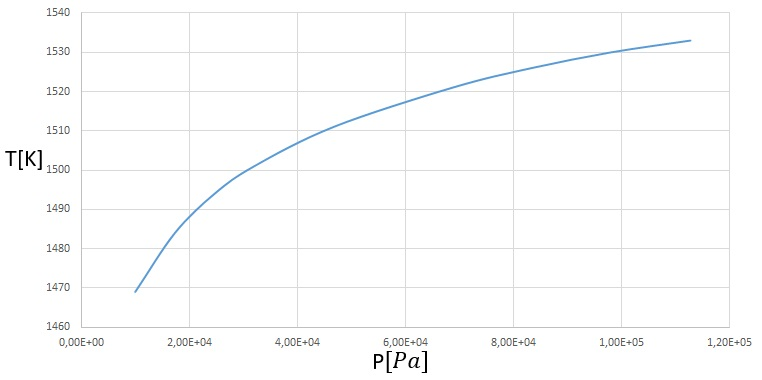
\includegraphics[width=1\textwidth]{1.jpg}
\caption{\label{fig:1}Temperature of an hydrogen-air ZND detonation in function of initial pressure from MATLAB calculations.}
\end{figure}

\begin{figure}[h!]
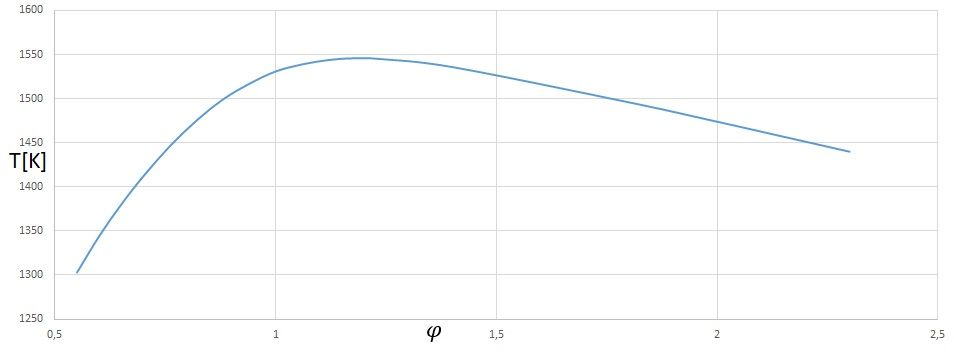
\includegraphics[width=1\textwidth]{2.jpg}
\caption{\label{fig:2}Temperature of an hydrogen-air ZND detonation in function of equivalence ratio from MATLAB calculations.}
\end{figure}

\begin{figure}[h!]
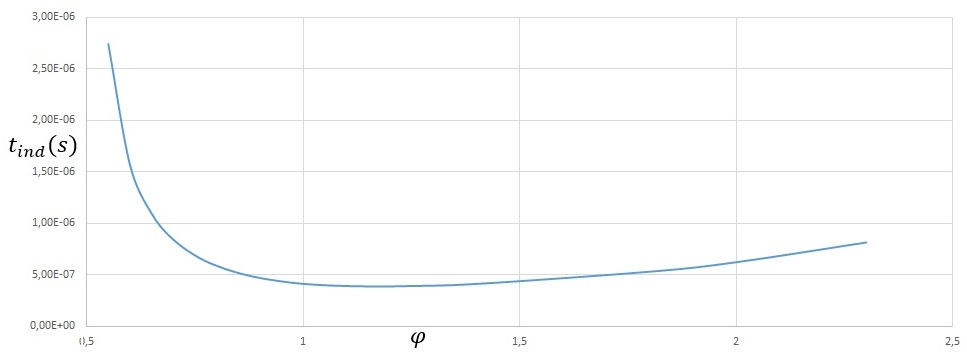
\includegraphics[width=1\textwidth]{3.jpg}
\caption{\label{fig:3}Induction time an hydrogen-air ZND detonation in function of equivalence ratio from MATLAB calculations.}
\end{figure}



The highest gradient of this time over equivalence ratio was  achieved at equivalence ratio 0.55-0.6.
$$\frac{dt_{ind}}{d\phi}=2,35∗10^{−5} _S$$
\\
\\
\\
According to research about detonation cell size, at these conditions minimal cell size equals 10mm at equivalence ratio of 1,18. This can be used to calculate the correlation between induced time and cell size.
$$\lambda =a ∗ t_{ind}$$
$$ a=\frac{\lambda}{t_{ind}}=\frac{10}{3,86∗10^{−7}}=2,59∗10^7 \frac{mm}{s}$$

\begin{figure}[h!]
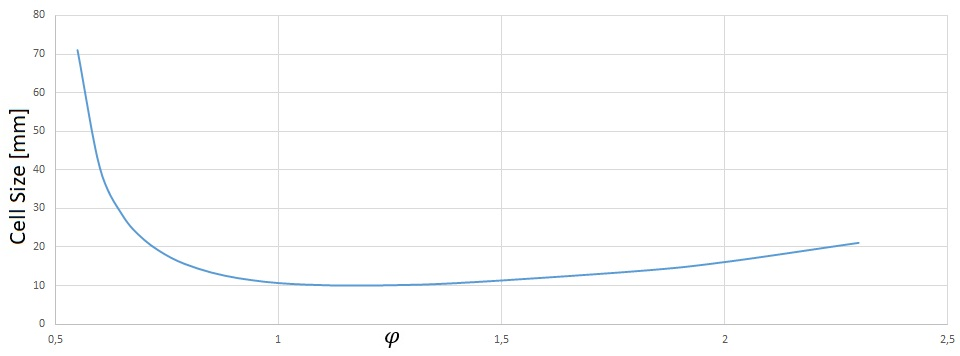
\includegraphics[width=1\textwidth]{4.jpg}
\caption{\label{fig:4}Calculated cell size}
\end{figure}

\begin{figure}[h!]
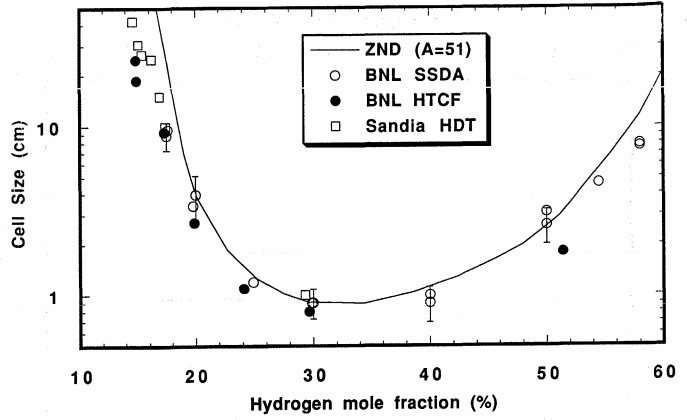
\includegraphics[width=1\textwidth]{5.jpg}
\caption{\label{fig:5}Cell size in function of fuel in air percentage. From source [2]}
\end{figure}
\newpage
\section{Conclusions}
Temperature of detonation rise with pressure, but temperature rise is get lower with increasing pressure. \newline The temperature of detonation has it maximum at equivalence ratio between 1,1 and 1,2. Both lower and higher equivalence ratio give lower temperatures. At side of poor mixtures it drop faster.\newline
According to research data calculation results have error not higher than 1\%. Both lower and higher equivalence ratio gave much higher mistake up to 15\%.

\section{References}

$
\hspace{5,35mm}[1] 
www.hysafe.net/wiki/BRHS/ChemicalPropertiesOfHydrogen
$

$
[2] www.osti.gov/scitech/servlets/purl/563843
$

$
[3] shepherd.caltech.edu/EDL/public/cantera/html/SD_Toolbox/
$

$
[4] en.wikipedia.org/wiki/ZND_detonation_model
$

$
[5] fluid.wme.pwr.wroc.pl/~spalanie/dydaktyka/spalanie_instrukcje/spalanie_labor_instr_stezeniowe_granice_palnosci_gazow.pdf
$

\end{document}